\chapter{Wobbling Motion in Nuclei}

The pioneering work of Bohr and Mottelson \cite{bohr1998nuclear} which was done more than 50 years ago lead to some interesting features regarding the collective phenomena in triaxial nuclei. Namely, they pointed out that a specific precessional motion of the nucleus's spin will take place when the rotational energy is sufficient. The angular momentum for triaxial nuclei is not aligned any of the principal axes of the ellipsoid, but it \emph{precesses} and \emph{wobbles} around one of these axes. They called this phenomenon \textbf{wobbling motion} (w.m.).
This combined motion comes from a consequence regarding the MOI. Indeed, the asymmetry of the three MOI makes the quantum mechanical nature of rotation to be possible around any of the three axes. As such, a \emph{main} rotation around the axis with the largest MOI will be the most energetically favorable, but the other two directions can \emph{quantum mechanically disturb} this main rotation, leading to this unique characteristic of triaxial nuclei.

The non-uniformity nature of w.m. was firstly studied for the `pure' rigid-rotators that correspond to the even-even nuclei. In this case, the w.m. can be treated as small amplitude oscillations of the total angular momentum $\mathbf{I}$ around the axis corresponding to the largest MOI.

\section{Wobbling Motion in Even-Even Nuclei}

The analytical expressions for wobbling excitations were firstly evaluated by Bohr and Mottelson using the so-called \emph{Harmonic Approximation} (HA). This can be described as a small-amplitude limit for the Triaxial Rigid Rotor Hamiltonian that was discussed in Chapter \ref{chapter4} (see Section \ref{trm-model}). In this limit, the projection of the total angular momentum onto the axis with largest MOI can be approximated $I_3\approx I$, meaning that the nucleus will do most of its rotation around this axis, with some `disturbance' from the other two principal of the triaxial rotor. 

For the description of this simple wobbler, one can consider the case when the $3$-axis has the largest MOI, and the following order holds true:
\begin{align}
    \mathcal{I}_3>\mathcal{I}_2>\mathcal{I}_1\ ,
\end{align}
or equivalently:
\begin{align}
    A_3<A_2<A_1\ .
\end{align}
The Hamiltonian can be written as:
\begin{align}
    \hat{H}_\text{rot}={\color{red}A_3I_3^2}+{\color{blue}\left(A_1I_1^2+A_2I_2^2\right)}
    \label{general-rotor-ham-evenA}
\end{align}

The different colors from Eq. \ref{general-rotor-ham-evenA} try to emphasize the fact that a Hamiltonian for the simple wobbler can be regarded as a main rotation around $3$-axis (represented by {\color{red}red color}) and the (precession + oscillation) of the total angular momentum (represented by {\color{blue}blue} color.)

The wobbling excitations which cause oscillations with small amplitudes for $\mathbf{I}$ about the $3$-axis are assumed to have a harmonic-like behavior, meaning that the final energy spectrum of a simple wobbler (even-even nucleus) will have the typical $\hbar\omega(n+1/2)$ behavior. Since this oscillator motion can be explained as `vibrations' of the total angular momentum around a steady position, where each wobbling excitation consists of an additional vibrating phonon, one can express the Hamiltonian in terms of \emph{boson} creation and annihilation operators. As such, the quantum mechanical treatment implies \cite{bohr1998nuclear}:
\begin{align}
    b^\dagger=\frac{1}{\sqrt{2I}}I_+\ ,\ b=\frac{1}{\sqrt{2I}}I_-\ ,\ \left[b,b^\dagger\right]\approx 1\ .
\end{align}

This initial quantization allows one to write Eq. \ref{general-rotor-ham-evenA} as a rotational term and a wobbling-specific one:
\begin{align}
    \hat{H}_\text{rot}&={\color{red}A_3I_3^2}+{\color{blue}H_w}\ ,\label{rot-ham-non-diagonal} \\
    {\color{blue}H_w}&={\color{blue}t_1\left(n+\frac{1}{2}\right)+\frac{1}{2}t_2(b^\dagger b^\dagger + bb)}\ ,
    \label{wob-ham-non-diagonal}
\end{align}
where the \emph{number of boson excitations} is denoted by $n$ and it is given by $n=b^\dagger b$. Each wobbling quanta will carry an angular momentum of one unit less with respect to the $3$-axis. The two factors $t_{1,2}$ are expressed in terms of the inertial parameters as \cite{bohr1998nuclear}:
\begin{align}
    t_1&=I(A_2+A_1-2A_3)\ , \\
    t_2&=I(A_2-A_1)\ .
\end{align}

Notice the linear dependence of the two parameters on the total angular momentum $I$. Moreover, depending on the values of $A_k$, the contribution of $t_{1,2}$ can be negative. Their behavior is shown within the right inset of Fig. \ref{fig-even-even-wobbling-energies}. Although the Hamiltonian $H_w$ is considered to have an oscillator-like behavior, its general expression does not look like a typical harmonic Hamiltonian. For this, the Hamiltonian given in Eq. \ref{wob-ham-non-diagonal} can be brought to a diagonalized form by introducing a new set of boson creation and annihilation operators. These operators will be written as linear combinations of $(b^\dagger,b)$:
\begin{align}
    c^\dagger=w_1b^\dagger-w_2b\ ,\\
    c=w_1b-w_2b^\dagger\ ,
\end{align}
where the two coefficients $w_{1,2}$ are defined in terms of $t_{1,2}$ as:
\begin{align}
    w_1&=\left[\frac{1}{2}\left(\frac{t_1}{\sqrt{t_1^2-t_2^2}}+1\right)\right]^{1/2}\ ,\nonumber\\
    w_2&=\left[\frac{1}{2}\left(\frac{t_1}{\sqrt{t_1^2-t_2^2}}+1\right)\right]^{1/2}\ .
    \label{eqs-w1-w2-terms-wobbling}
\end{align}

The terms $w_{1,2}$ are verify the condition $w_1^2-w_2^2=1$ and they make the `dangerous' products ($b^\dagger b^\dagger$,$bb$) disappear in this new representation \cite{oi2006semi}. Note that there is no spin dependence inferred in Eq. \ref{eqs-w1-w2-terms-wobbling} such that $w_{1,2}$ are constant functions of spin, unlike the coefficients $t_{1,2}$. Moreover, introducing a number operator $\hat{n}=c^\dagger c$ and the excitation quanta $\hbar\omega_w$ defined as:
\begin{align}
    \hbar\omega_w=\sqrt{t_1^2-t_2^2}=2I\sqrt{(A_1-A_3)(A_2-A_3)}\ ,
    \label{wobbling-frequency-even-A}
\end{align}
then a final expression of $H_w$ can be expressed, which has a behavior typical to the \emph{harmonic oscillator}:
\begin{align}
    H_w=\hbar\omega_w\left(\hat{n}+\frac{1}{2}\right)\ .
    \label{wob-ham-diagonal}
\end{align}

In this expression, the excitation quanta $\hbar\omega_w$ which was defined in Eq. \ref{wobbling-frequency-even-A} in terms of $t_{1,2}$ is called \emph{wobbling frequency} and its increasing linearly with the total angular momentum. Accordingly, Eq. \ref{rot-ham-non-diagonal} can be re-written with the wobbling Hamiltonian defined in Eq. \ref{wob-ham-diagonal}:
\begin{align}
    \hat{H}_\text{rot}=A_3I(I+1)+\hbar\omega_w\left(\hat{n}+\frac{1}{2}\right)\ .
    \label{rot-wob-ham-diagonal}
\end{align}

Thus, in the HA, the eigenvalues of the rotor Hamiltonian can be expressed in terms of a \emph{wobbling phonon number} $n_w$ (which is the eigenvalue of the number operator $\hat{n}=c^\dagger c$) and a \emph{wobbling frequency} (defined in Eq. \ref{wobbling-frequency-even-A}):
\begin{align}
    E_{I,n}={\color{red}A_3I(I+1)}+{\color{blue}\hbar\omega_w\left(n_w+\frac{1}{2}\right)}\ .
    \label{eq-wobbling-energy-evenA}
\end{align}

The spectrum for an even-even wobbling nucleus is thus represented by Eq. \ref{eq-wobbling-energy-evenA}. Notice again the two colored terms that illustrate the energy coming from the rotation around the $3$-axis and the disturbed motion with small oscillations around the other two axes. Consequently, the wobbling character of the system will be generated by the latter harmonic term. The wobbling phonon number $n_w$ is related to the `strength' of the tilting for $\mathbf{I}$, indicating the fact that an increasing number for $n_w$ will result in oscillations with larger amplitudes around the other two axes. The phonon number takes values $n_w=0,1,\dots$. In Fig. \ref{wobbling-geometry-tilting-sketch}, a sketch which shows the tilting effect that the wobbling phonon number has on the total angular momentum vector is drawn, together with a typical band structure for wobbling motion.

\begin{figure}
    \centering
    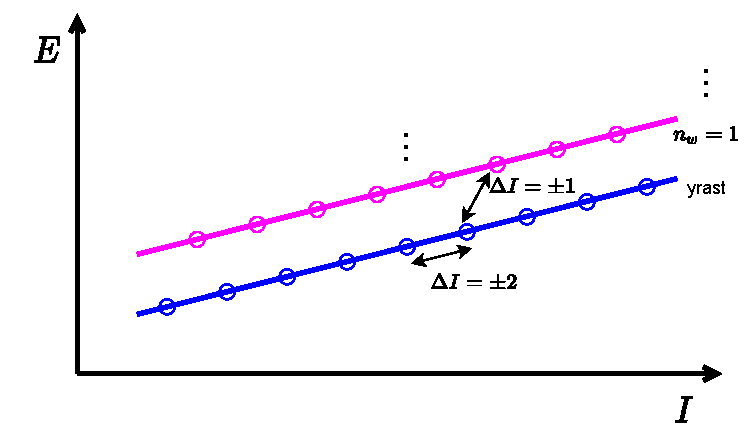
\includegraphics[scale=0.3]{Chapters/Figures/wobbling_n_schematic-1.pdf}
    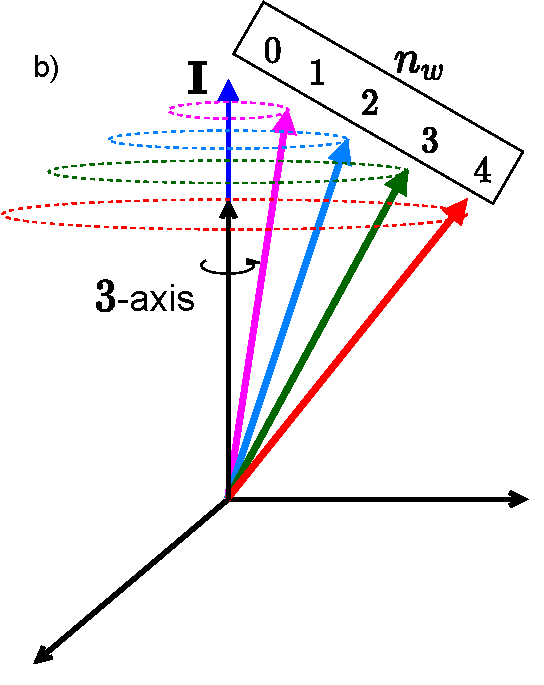
\includegraphics[scale=0.3]{Chapters/Figures/wobbling_n_schematic-2.pdf}
    \caption{caption}
    \label{wobbling-geometry-tilting-sketch}    
\end{figure}

As a quantitative analysis of the wobbling frequency and the rotor energy, one can take three arbitrary values for the moments of inertia (and, implicitly, the inertia factors $A_k$) and see the behavior of both $E_{I,n}$ and $\hbar\omega_w$ with increasing angular momentum and wobbling phonon number. Keep in mind that depending on the value of the wobbling phonon number, different spin sequences will be allowed. More precisely, from the invariance of the rotor w.r.t. rotations by $\pi$ about the principal axes for even-even nuclei, the signature quantum number $\alpha$ can take the values 0 and 1. Each wobbling band will have an alternating signature, starting with $\alpha=0$ for $n_w=0$ then $\alpha=1$ for $n_w=1$ and so on: even spin sequences appear for even values of $n_w$ and odd spin sequences appear for odd values of $n_w$ (see Fig. \ref{wobbling-geometry-tilting-sketch}).

The rotor energy from Eq. \ref{eq-wobbling-energy-evenA} is graphically represented for an arbitrary set of moments of inertia as a function of the nuclear angular momentum $I$ in Fig. \ref{fig-even-even-wobbling-energies}. This pedagogical example contains rotational bands up to $n_w=5$ in the wobbling phonon number. From Fig. \ref{fig-even-even-wobbling-energies}, one can see the linear dependence on the total angular momentum and, moreover, the wobbling energy and frequency both are increasing with spin.

\begin{figure}
    \centering
    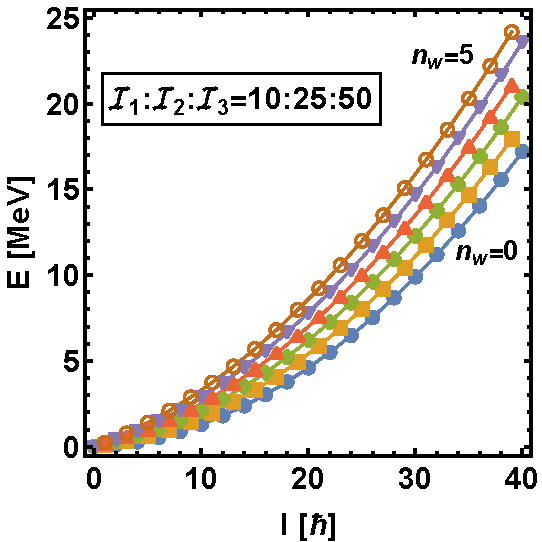
\includegraphics[scale=0.7]{Chapters/Figures/wobbling-evenA.pdf}
    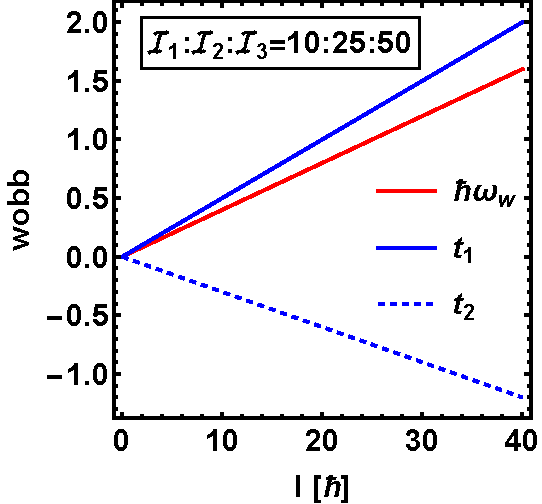
\includegraphics[scale=0.74]{Chapters/Figures/wobblingFreq-evenA.pdf}
    \caption{\textbf{Left:} The energy spectrum for an even-even nucleus with three different moments of inertia, with the main rotation around the $3$-axis, according to Eq. \ref{eq-wobbling-energy-evenA}. Each wobbling band has alternating signature number $\alpha$ (starting with $\alpha=0$ for the ground state $n_w=0$ band). Notice the even/odd spin sequences for each band. \textbf{Right:}: The wobbling frequency plotted together with the linear terms $t_1$ and $t_2$ that are used to express $\hbar\omega_w$. Same set of MOI were used across both figures and the unit for $\mathcal{I}_i$ is $\hbar^2\ \text{MeV}^-1$.}
    \label{fig-even-even-wobbling-energies}
\end{figure}


Another instructive analysis would be the evolution of the components of $\mathbf{I}$ as a function of the polar and azimuthal angles $\theta,\varphi$. Indeed, expressing the three components as:
\begin{align}
    I_1&=I'\sin\theta\cos\varphi\ ,\\
    I_2&=I'\sin\theta\sin\varphi\ ,\\
    I_3&=I'\cos\theta\ ,
    \label{angular-momentum-polar-components}
\end{align}
where $I'=\sqrt{I(I+1)}$, one can make a graphical representation for these components. In Fig. \ref{figs-angular-momentum-components-polar}, the components $I_1$ and $I_2$ are represented in the $\theta,\varphi$ plane, for a fixed value $I=10\hbar$. Since the third component is independent of the azimuthal angle $\varphi$, it has been dismissed.

\begin{figure}
    \centering
    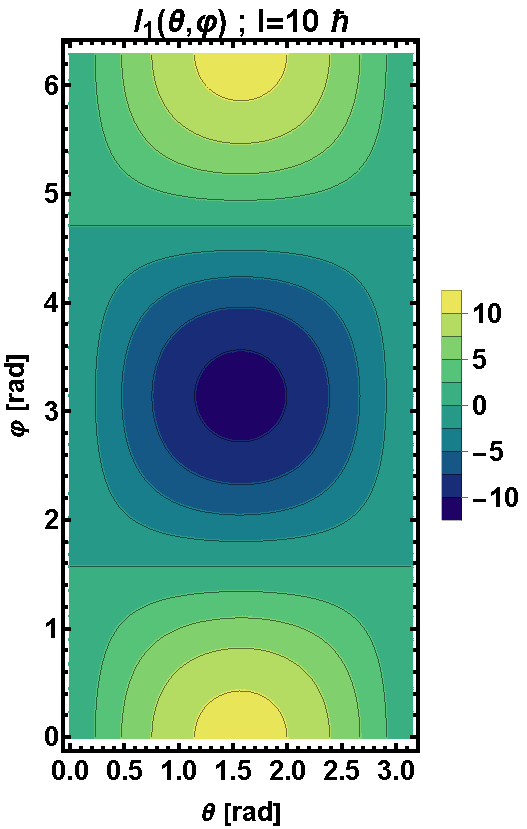
\includegraphics[scale=0.66]{Chapters/Figures/angular_components-TRM-1.pdf}
    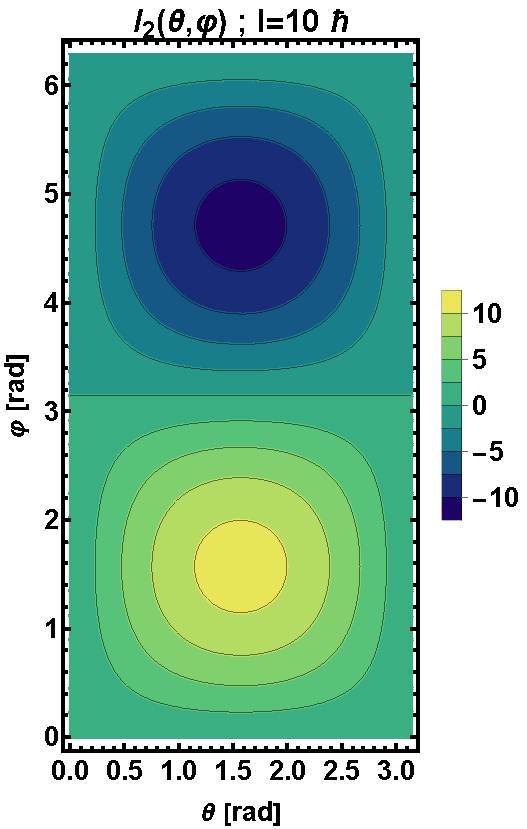
\includegraphics[scale=0.66]{Chapters/Figures/angular_components-TRM-2.pdf}
    \caption{The geometrical representation of the first and second component of the total angular momentum $\mathbf{I}$, as function of the polar angles, according to Eq. \ref{angular-momentum-polar-components}.}
    \label{figs-angular-momentum-components-polar}
\end{figure}

The other relevant observables which can be calculated for simple wobbler within the HA are the two quadrupole moments $Q_{20,22}$ and the intraband + interband $B(E2)$ transition probabilities. The quadrupole components are expressed in terms of the intrinsic quadrupole moment $Q_0$ and the triaxiality parameter as \cite{shoji2006microscopic}:
\begin{align}
    Q_{20}=Q_0\cos\gamma\ ,\ Q_{22}=\frac{1}{\sqrt{2}}Q_0\sin\gamma\ .
\end{align}

These components can be furthermore used to determine the intraband $B(E2)$ transition probabilities \cite{wen2015wobbling}:
\begin{align}
    B(E2;(n,I)\to(n,I-2))=\frac{5}{16\pi}Q_{22}^2\ ,
\end{align}
and also the interband transitions:
\begin{align}
    B(E2;(n,I)\to(n-1,I-1))&=\frac{5}{16\pi}\frac{n}{I}\left(\sqrt{3}Q_{20}w_1+\sqrt{2}Q_{22}w_2\right)^2\ ,\\
    B(E2;(n,I)\to(n+1,I-1))&=\frac{5}{16\pi}\frac{n+1}{I}\left(\sqrt{3}Q_{20}w_2+\sqrt{2}Q_{22}w_1\right)^2\ .
\end{align}

\subsubsection*{Triaxial rotor energy vs. wobbling energy}

An important discussion should be made regarding the nomenclature for energies when referring to wobbling motion. As shown in Eq. \ref{eq-wobbling-energy-evenA}, the energy spectrum for a simple wobbler can be determined for every phonon number and spin sequences. However, that is the `full' spectrum which is composed of the \emph{yrast} states with $n_w=0$ and the \emph{excited states} having $n_w=1,\dots$. On the other hand, the so-called `wobbling energies' are defined in terms of these values $E_{I,n}$ with the following rules \cite{wen2015wobbling}:
\begin{align}
    E_\text{wob}(I_\text{even})&=E_{I,n}-E_{I,0}\, \\
    E_\text{wob}(I_\text{odd})&=E_{I,n}-\frac{1}{2}\left(E_{I-1,0}+E_{I+1,0}\right)\, 
\end{align}
where the former wobbling energy corresponds to the even values of $I$ and the latter is applied for odd values of $I$. Within the literature, the wobbling spectrum/energy is often referred to the entire structure \ref{eq-wobbling-energy-evenA}, so one has to be careful.

\subsection{Testing the Harmonic Approximation}

It is worth going further and apply the formalism for even-even nuclei within the Harmonic Approximation for an existing spectrum. As such, one can take $^{130}$Ba as a testing example. As it will be discussed, it turns out that experimentally, the wobbling structures in even-mass isotopes have been very scarce. Very recently Petrache et al. \cite{petrache2019diversity} identified a large collection of band structures in $^{130}$Ba. Two of them are reported to be of wobbling nature \cite{chen2019transverse}.